\documentclass[12pt]{report} 
\usepackage{graphicx}
\usepackage{wrapfig}
\usepackage{placeins}

\usepackage{graphicx}
\usepackage[table]{xcolor}
\usepackage{amsmath}
\usepackage{cancel} 
\usepackage{placeins}
\usepackage{hyperref}
\usepackage{url}
\usepackage{multicol}
\usepackage{booktabs}
\usepackage[toc,page]{appendix}
\usepackage{glossaries}
%\makenoidxglossaries

\newacronym{cdr}{CDR}{Creighton Digital Repository}


\newacronym{hrs}{HRS}{Heart Rhythm Society}
\newacronym{cied}{CIED}{cardiac implantable electronic device}
\newacronym{icd}{ICD}{implantable cardioverter-defibrillators}
\newacronym{crt}{CRT}{cardiac resynchronization therapy}
\newacronym{ecg}{ECG}{electrocardigram}



\newacronym{rf}{RF}{radiofrequency}
\newacronym{dac}{DAC}{data acquisition card}
\newacronym{pd}{PD}{Proton Density}
\newacronym{pla}{PLA}{Polylactic Acid}
\newacronym{pvc}{PVC}{Polyvinyl Chloride}
\newacronym{lvi}{VI}{LabVIEW Virtual Instrument}
\newacronym{mri}{MRI}{Magnetic Resonance Imaging}

\definecolor{steelblue}{rgb}{0.27, 0.51, 0.71}
\definecolor{crimson}{rgb}{0.86, 0.08, 0.24}
\definecolor{darkslategray}{rgb}{0.18, 0.31, 0.31}

\hypersetup{colorlinks   = true, %Colours links instead of ugly boxes
	urlcolor     = steelblue, %Colour for external hyperlinks
	linkcolor    = darkslategray, %Colour of internal links
	citecolor   = crimson %Colour of citations
    }
\renewcommand\bibname{References}
\usepackage{setspace}
\usepackage[letterpaper,left=1.5in,right=1in,top=1in,bottom=1in]{geometry}

\usepackage{pdflscape}
%\usepackage{subfigure}
\usepackage{subcaption}
\usepackage{float}
\usepackage{wrapfig}
\usepackage{pdfpages}
\widowpenalty10000% This automatically groups lines so there is at least 2 from each paragraph on a page.  Optional
\clubpenalty10000 %see above comment
\usepackage{indentfirst} %This makes the first paragraph of a section indented.  Optional.
\usepackage{breqn}

\setcounter{secnumdepth}{4}
\setcounter{tocdepth}{4}



\newlength{\subcolumnwidth}
\newenvironment{subcolumns}[1][0.45\columnwidth]
{\valign\bgroup\hsize=#1\setlength{\subcolumnwidth}{\hsize}\vfil##\vfil\cr}
{\crcr\egroup}
\newcommand{\nextsubcolumn}[1][]{%
	\cr\noalign{\hfill}
	\if\relax\detokenize{#1}\relax\else\hsize=#1\setlength{\subcolumnwidth}{\hsize}\fi
}
\newcommand{\nextsubfigure}{\vfill}

\begin{document}
	
\begin{figure}[hbt!]
		\centering
		\subfloat[PVC-based mapping platform.\label{fig:fieldmapping_a}]{
			
\includegraphics[width=0.48\textwidth]{rulerZoom.jpeg}
		}
		\hfill
		\subfloat[Example field map output from MRI fringe region.\label{fig:fieldmapping_b}]{
			
\includegraphics[width=0.40\textwidth]{rulerZoom.jpeg}
		}
		
		\caption[PVC-based magnetic field mapping platform]{PVC-based magnetic field mapping platform. Used for spatial $B_0$ and $\nabla B_0$ measurement. based on design from Ferreira, et al. (2017) \cite{haddixProposal,ferreira2017}.}
		\label{fig:fieldmapping}
\end{figure}

 Panel (a) shows the full assembly. Panel (b) highlights the upper ring designed to secure the pendulum string. Panel (c) shows the lower ring containing the slit used to align a 1cm-wide ruler for displacement measurements.

\begin{figure}[htbp]
	\centering
	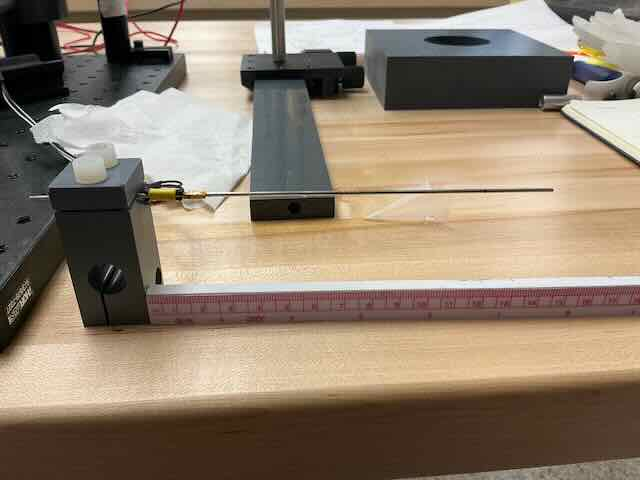
\includegraphics[width=0.7\textwidth, keepaspectratio]{sensorResting.jpeg}
	\caption[Temperature vs. Reaction Rate]{Temperature dependence of 
		the reaction rate for catalyst A. Error bars represent standard 
		deviation from three independent measurements (n=3).}
	\label{fig:temp-rate}
\end{figure}
	
\begin{figure}[htbp]
	\centering
	% First row
	\begin{subfigure}{0.3\textwidth}
		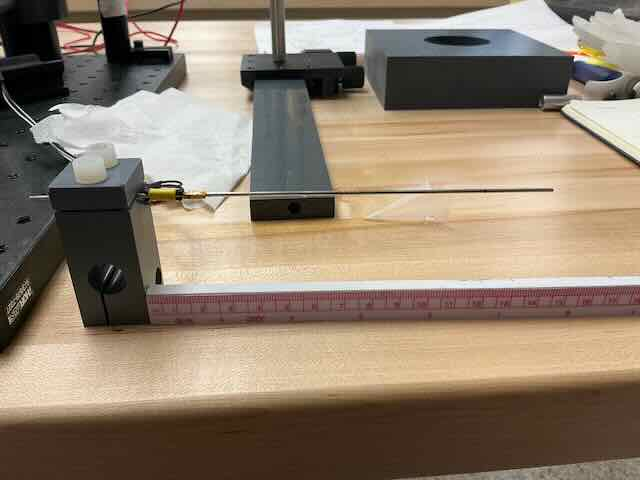
\includegraphics[width=\textwidth]{sensorResting.jpeg}
		\caption{Condition A}
	\end{subfigure}
	\hfill
	\begin{subfigure}{0.3\textwidth}
		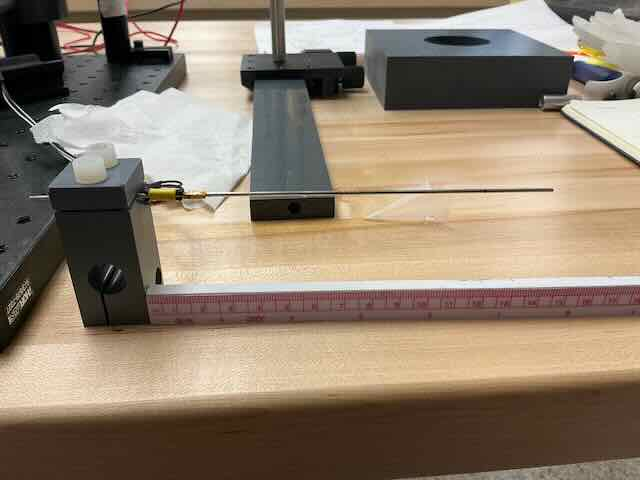
\includegraphics[width=\textwidth]{sensorResting.jpeg}
		\caption{Condition B}
	\end{subfigure}
	\hfill
	\begin{subfigure}{0.3\textwidth}
		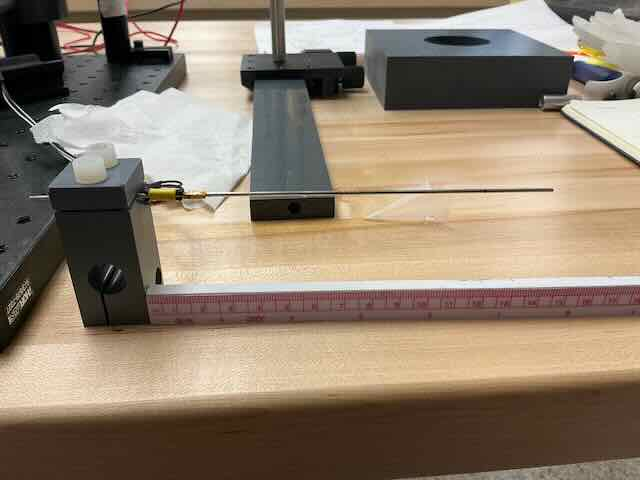
\includegraphics[width=\textwidth]{sensorResting.jpeg}
		\caption{Condition C}
	\end{subfigure}
	
	\vspace{0.5cm} % Vertical space between rows
	
	% Second row
	\begin{subfigure}{0.3\textwidth}
		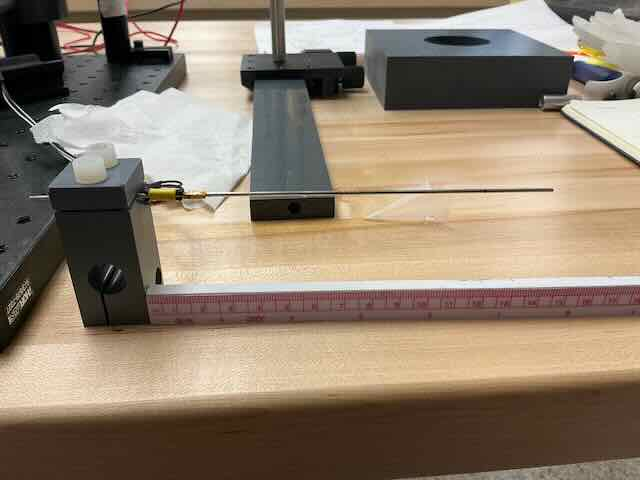
\includegraphics[width=\textwidth]{sensorResting.jpeg}
		\caption{Result A}
	\end{subfigure}
	\hfill
	\begin{subfigure}{0.3\textwidth}
		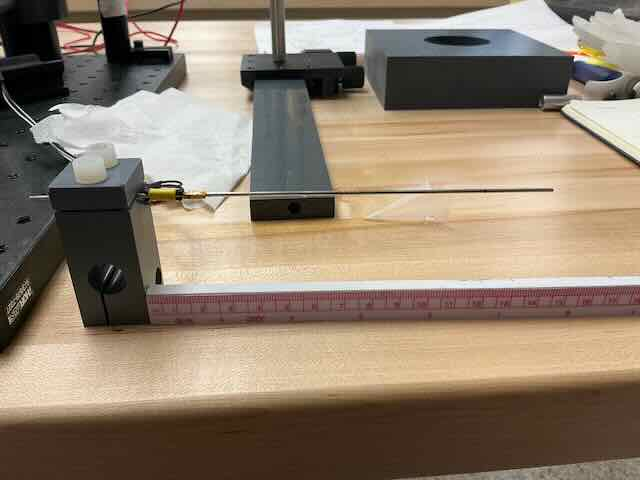
\includegraphics[width=\textwidth]{sensorResting.jpeg}
		\caption{Result B}
	\end{subfigure}
	\hfill
	\begin{subfigure}{0.3\textwidth}
		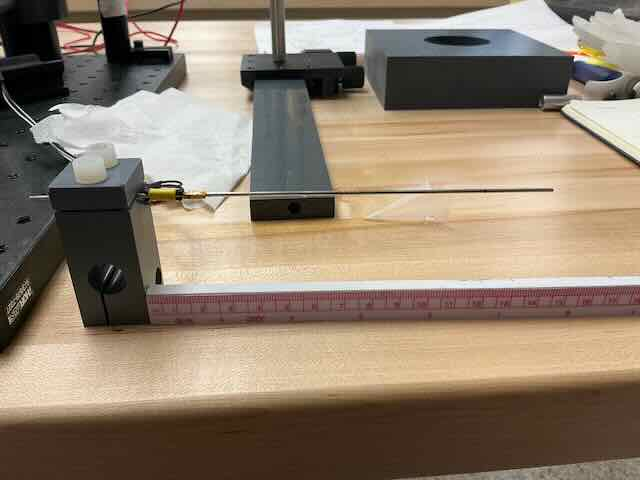
\includegraphics[width=\textwidth]{sensorResting.jpeg}
		\caption{Result C}
	\end{subfigure}
	
	\caption{Comparison of experimental conditions and their results.}
\end{figure}	



\begin{figure}[htbp]
	\centering
	\begin{subfigure}{0.45\textwidth}
		\centering
		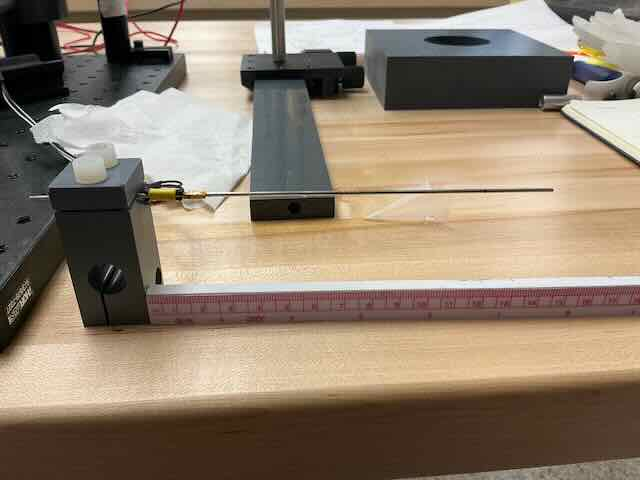
\includegraphics[width=\textwidth]{sensorResting.jpeg}
		\caption{First subfigure}
		\label{fig:sub1}
	\end{subfigure}
	\hfill % Adds horizontal space between subfigures
	\begin{subfigure}{0.45\textwidth}
		\centering
		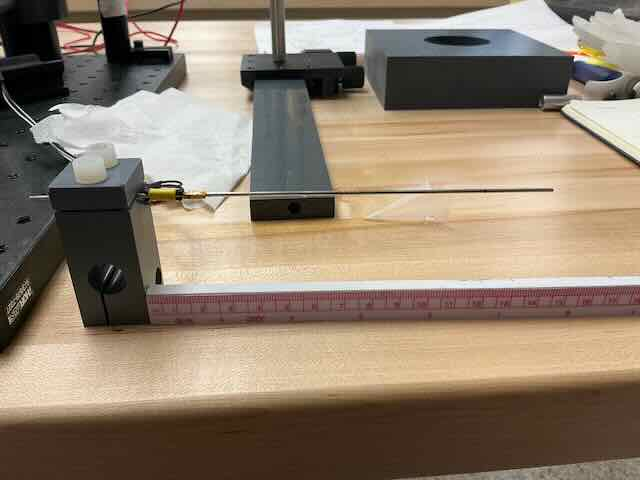
\includegraphics[width=\textwidth]{sensorResting.jpeg}
		\caption{Second subfigure}
		\label{fig:sub2}
	\end{subfigure}
	\caption{Main caption for the complete visual.}
	\label{fig:main}
\end{figure}

\begin{wrapfigure}{r}{0.4\textwidth}
	\centering
	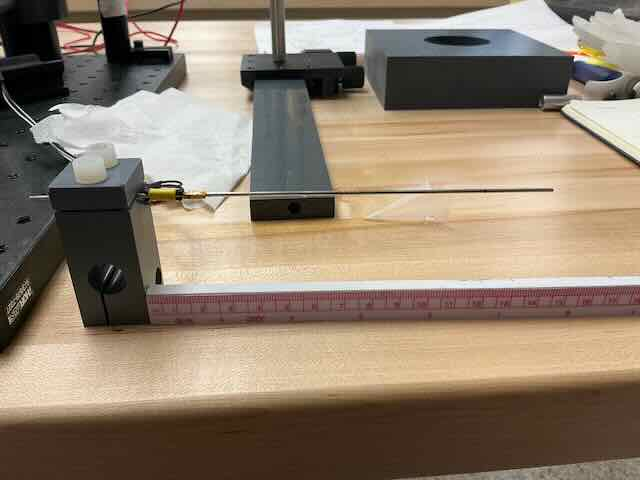
\includegraphics[width=0.35\textwidth]{sensorResting.jpeg}
	\caption{Figure with text wrapping.}
\end{wrapfigure}
This text will wrap around the figure on the right side of the page, 
continuing until the bottom of the figure is reached. Additional 
paragraphs will continue wrapping naturally. This text will wrap around the figure on the right side of the page, 
\FloatBarrier
continuing until the bottom of the figure is reached. Additional 
paragraphs will continue wrapping naturally. This text will wrap around the figure on the right side of the page, 
continuing until the bottom of the figure is reached. Additional 
paragraphs will continue wrapping naturally.

  \begin{figure}[!htb]
	\centering
	\begin{subfigure}[b]{0.45\textwidth}
		
\includegraphics[angle=-90,width=1.2\textwidth, keepaspectratio]{TransFix.jpg}
		\caption{First}\label{subfig-1:dummy}
	\end{subfigure}
	\hfill
	\begin{minipage}[b]{0.45\textwidth}
		\begin{subfigure}[b]{\linewidth}
		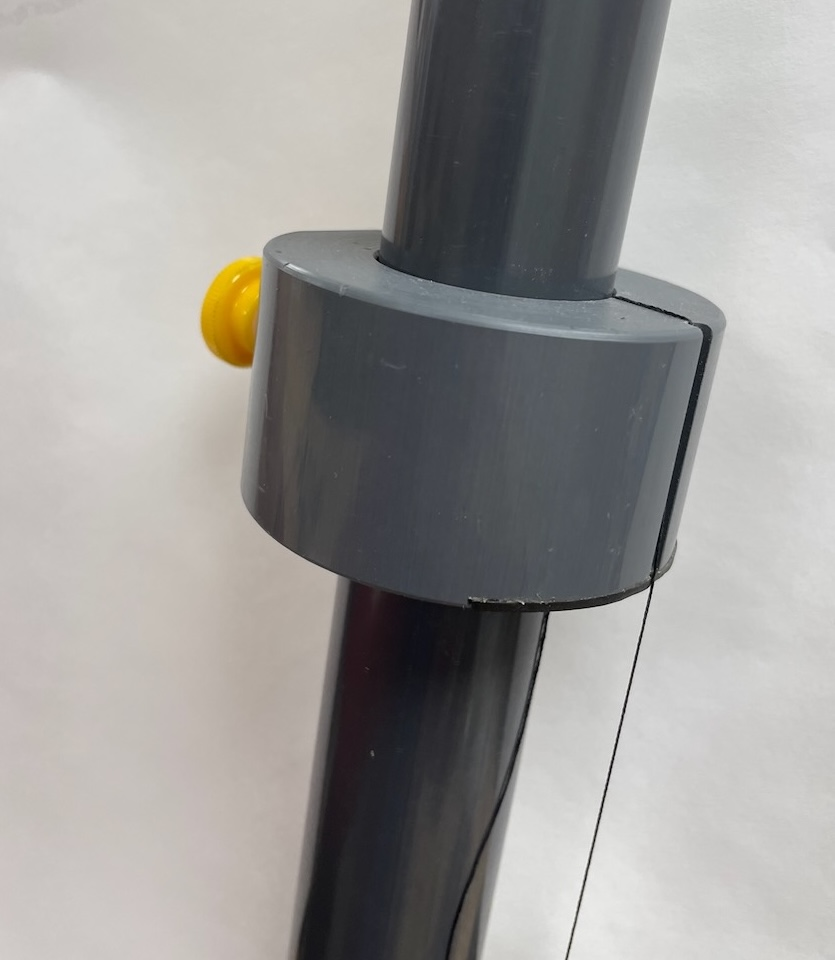
\includegraphics[width=0.7\textwidth, keepaspectratio]{stringZoom.jpeg}
			\caption{Second}\label{subfig-2:dummy}
		\end{subfigure}\\[\baselineskip]
		\begin{subfigure}[b]{\linewidth}
		
\includegraphics[width=0.7\textwidth, keepaspectratio]{rulerZoom.jpeg}
			\caption{Third}\label{subfig-3:dummy}
		\end{subfigure}
	\end{minipage}
	\caption{Dummy figure}\label{fig:dummy}
\end{figure}


\begin{figure}[!htp]
\centering
	\begin{minipage}{.9\textwidth}
		\begin{subcolumns}[0.61\textwidth] %ancho de primera columna
			
			\subfloat[Full view of the constructed pendulum fixture.\label{fig:realpendulum_full}]{
\includegraphics[angle=-90,width=\subcolumnwidth]{TransFix.jpg}}
			
			\nextsubcolumn[0.31\textwidth] %ancho de segunda columna
			
			\subfloat[Upper ring close-up with clamp and rubber attachment.\label{fig:realpendulum_upper}]{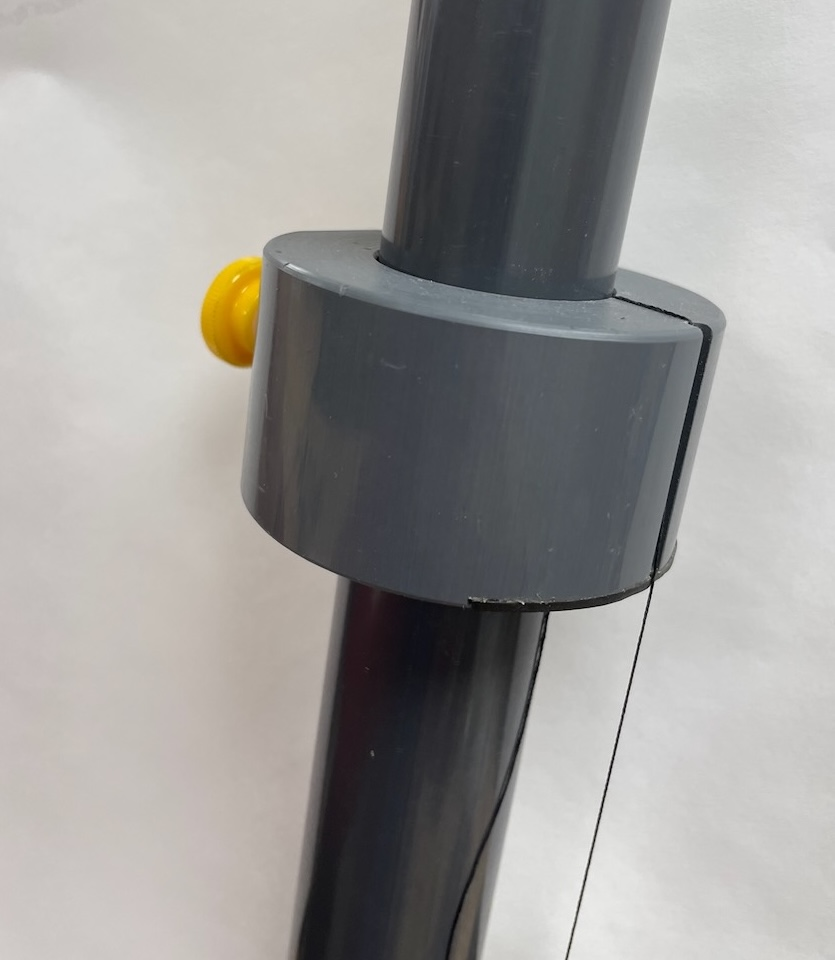
\includegraphics[width=\subcolumnwidth]{stringZoom.jpeg}}
			
			\nextsubfigure
			
		\subfloat[Lower ring close-up with horizontal 20 cm ruler.\label{fig:realpendulum_lower}]{
\includegraphics[width=\subcolumnwidth]{rulerZoom.jpeg}}
			
		\end{subcolumns}
	\end{minipage}
	\caption{Global caption}
\end{figure}

\begin{figure}[H]
	\centering
	
	\subfloat[Voltage readings for Rod5 (Glass) with up to 750 mg of water in increments.\label{fig:glassRod5}]{
		
\includegraphics[width=0.46\textwidth]{rulerZoom.jpeg}
	}
	\hfill
	\subfloat[Voltage readings for Rod7 (Clear Plastic) with up to 800 mg of water in increments..\label{fig:clearRod7}]{
		
\includegraphics[width=0.46\textwidth]{rulerZoom.jpeg}
	}
	\caption[Calibration trial results for low-torque rods showing poor sensor response]{Trial examples for Rods 5 and 7. Both of them showed inconsistency across trials showing minimal to no change in voltage with weight added.}
	\label{fig:rods5n7}
\end{figure}

\begin{figure}[htb!]
	\centering
	
	\subfloat[Curve fit of measured pendulum deflection vs. applied magnetic force.\label{fig:curve_fit_plot}]{
		
\includegraphics[width=0.9\textwidth]{rulerZoom.jpeg}
	}
	\hfill
	\subfloat[Residuals from linear fit of $\tan(\alpha)$ vs. $B_0 \cdot \frac{dB_0}{dz}$. Error bars indicate propagated uncertainties.\label{fig:residuals_plot}]{
		
\includegraphics[width=0.9\textwidth]{rulerZoom.jpeg}
	}
	\caption[Residuals and curve fit comparison]{: (a) residuals from the linearized fit, and (b) fitted curve against the measured data points.}
	\label{fig:fit}
\end{figure}

\end{document}